\chapter{Realizability}
\label{chap:realizability}

\section{Basic definitions}
\label{sec:basic-definitions}

\subsection{Motivation and the basic idea}
\label{sec:realizability-basic-idea}

Realizability was introduced by Stephen Kleene~\cite{KleeneSC:intint}
who used it to build a model of intuitionistic arithmetic. Our purpose
is to study not only the theoretical aspects of computable
mathematics, but also practical issues. Thus we approach realizability
by asking a practical question: given a mathematical structure
(constants, functions, relations, and axioms), what should a computer
implementation look like? For simple cases, the answer is obvious. A
group would have a type whose values represent group elements, a value
representing the neutral element, and functions which compute the
group operation and inverses. But for more interesting structures,
especially those arising in mathematical analysis, the answer is less
clear. How do we implement the real numbers (and we do not mean
floating-point arithmetic, we mean the \emph{real} real numbers)?
Which operations on a compact metric space can be implemented? How do
we implement a space of smooth functions? Significant research goes
into finding satisfactory answers to such
questions~\cite{Wei00,TZ98,Bla97}.

To explain the basic idea behind realizability we consider a small
real-world programming example. Suppose we are asked to design a data
structure for the set $\mathsf{Graphs}$ of all finite
simple\footnote{Simple means at most one arrow between any two
  vertices.} directed graphs with vertices labeled by distinct
integers. An typical such graph~$G$ is shown in
Figure~\ref{fig:digraph}.
%
\begin{figure}[htp]
  \centering
  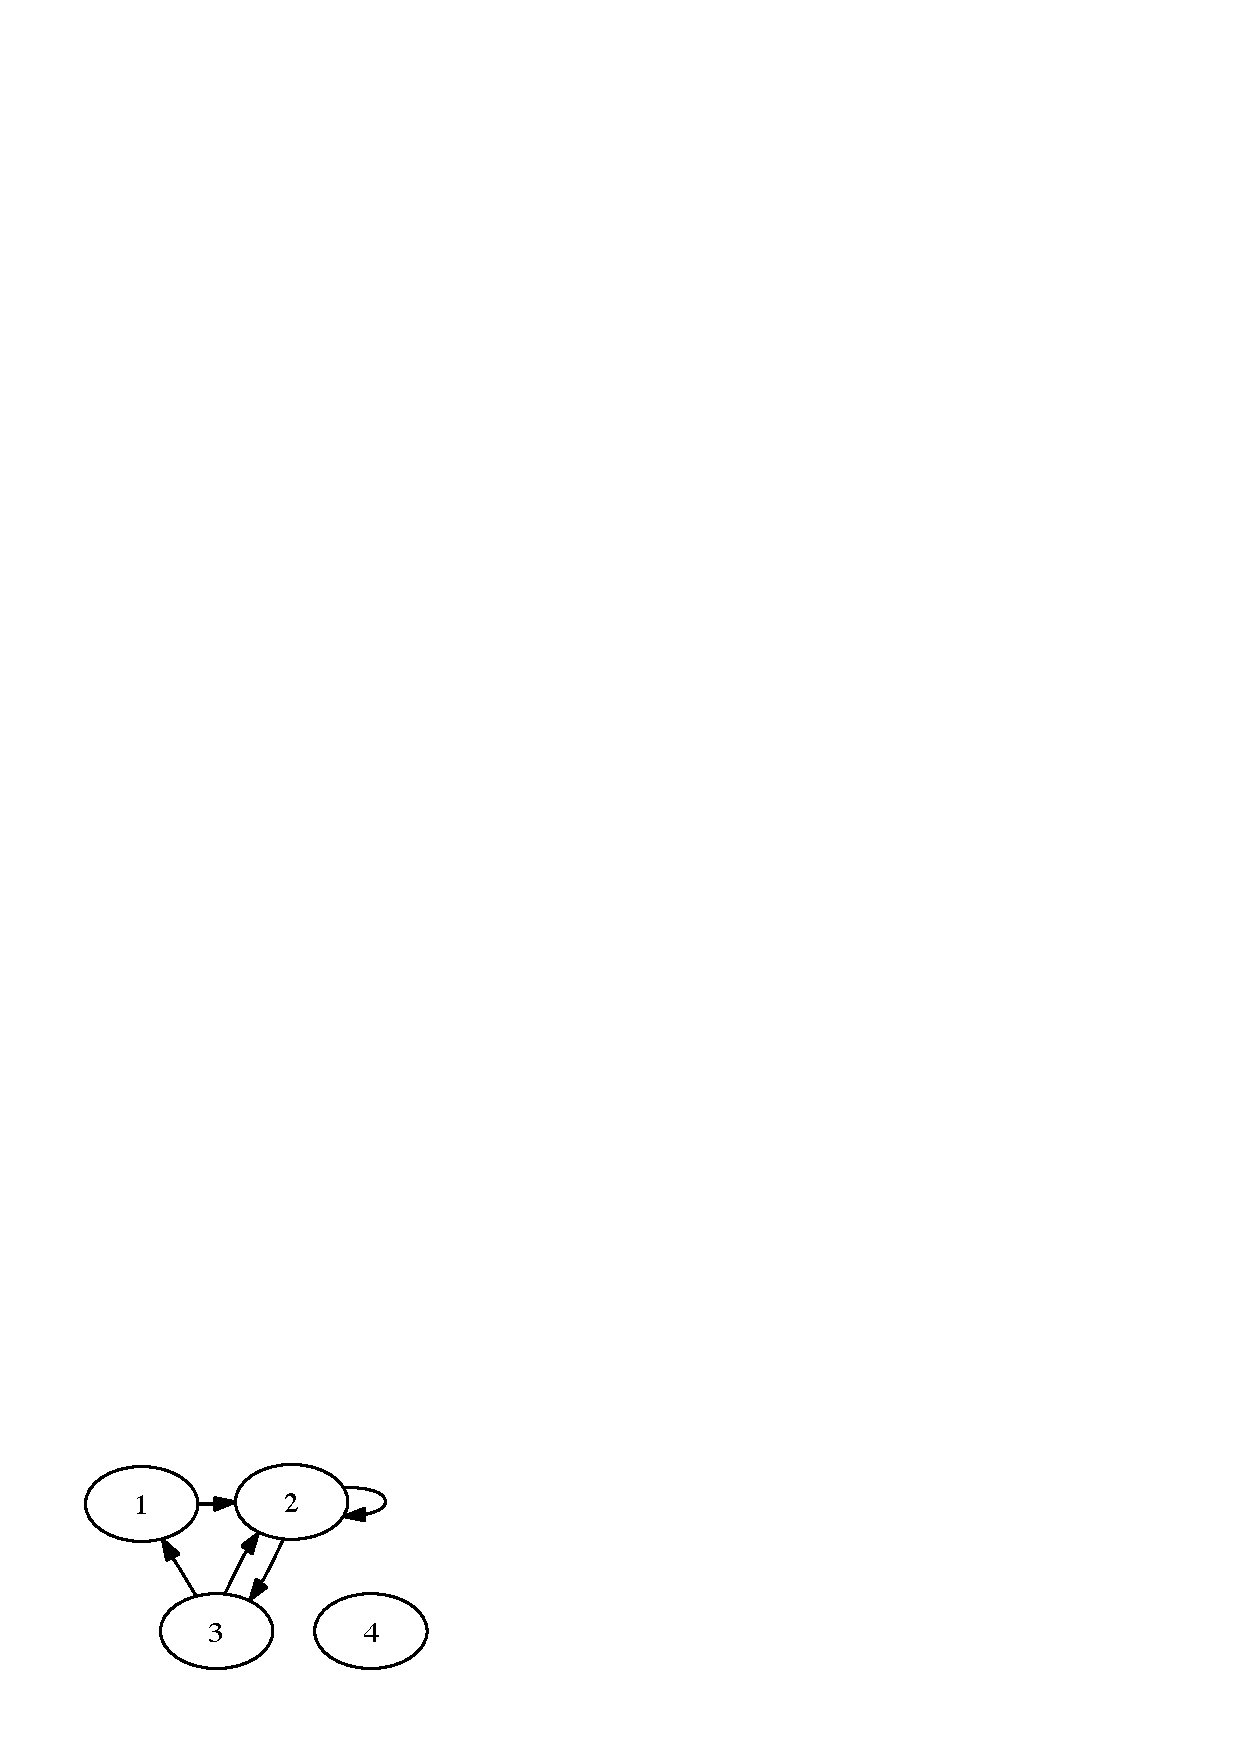
\includegraphics[width=0.3\textwidth]{digraph}
  \caption{A finite directed graph $G$}
  \label{fig:digraph}
\end{figure}
%
One common representation of such graphs uses a pair of lists
$(\ell_V, \ell_A)$, where $\ell_V$ is the list of vertex labels and
$\ell_A$ is the \emph{adjacency list} representing the arrows by
pairing the labels of each source and target. For the above graph $G$,
$\ell_V = [1, 2, 3, 4]$ and $\ell_A = [(1,2), (2,2), (2,3), (3,2),
(3,1)]$.
%
Thus we define the datatype of graphs as\footnote{We use Haskell
  notation in which $[t]$ is the type of lists of elements of
  type~$t$, and $(t_1, t_2)$ is the cartesian product of types~$t_1$
  and~$t_2$.}
%
\begin{lstlisting}[language=Haskell]
type Graph = ([Int], [(Int, Int)])
\end{lstlisting}
%
However, this is not a complete description of the intended
representation, as there are representation invariants and conditions
not expressed by the type, e.g.,
%
\begin{enumerate}
\item The order in which vertices and arrows are listed is not
  important%
; for example, $[1,2,3,4]$ and $[4,1,2,3]$ represent the same vertices.
\item Each vertex and arrow must be listed exactly once.
\item The source and target of each arrow must appear in the list of vertices.
\end{enumerate}
%
Consequently, to fully implement the mathematical
set~$\mathsf{Graphs}$ we must not only decide on the underlying
datatype $\mathtt{graph}$, but also determine what values of that type
represent which elements of~$\mathsf{Graphs}$. All this can be
expressed with a \emph{realizability relation}
%
\begin{equation*}
  r \rz x
\end{equation*}
%
which is read as ``$r$ realizes $x$''. In the above example we would
write
%
\begin{equation*}
([1, 2, 3, 4], [(1,2), (2,2), (2,3), (3,2), (3,1)]) \rz G.
\end{equation*}
%
Once the set $\mathsf{Graphs}$ is implemented as a datatype, an
obvious thing to do is to compute with it. When can we say that a
function $f : \mathsf{Graphs} \to \mathsf{Graphs}$ is computable? The
answer again is quite natural for a programmer: $f$ is computed by a
program $p : \mathtt{graph} \to \mathtt{graph}$ when $p$ does to
realizers what $f$ does to elements: if $r \rz G$ then $p(r) \rz
f(G)$. We say that the map $f$ is \emph{realized} or \emph{tracked} by
the program~$p$.


\subsection{Assemblies}
\label{sec:assemblies}

We now give a precise definition of the ideas presented in the
previous section.

\begin{definition}[Assemblies]
  Let $A$ be a TPCA and $\comp{A}$ a sub-TPCA. An \emph{assembly}
  over~$(A, \comp{A})$ is a triple $(S, |S|, {\rz_S})$ where $S$ is a
  set, $|S|$ is a type, and $\rz_S$ is a relation between $A_{|S|}$
  and~$S$ satisfying: for every $x \in S$ there is $r \in A_{|S|}$
  such that $r \rz_S x$.

  A \emph{realized map} $f : S \to T$ between assemblies $(S, |S|,
  {\rz_S})$ and $(T, |T|, {\rz_T})$ is a map for which there exists $p
  \in \comp{A}_{|S| \to |T|}$ satisfying: if $r \rz_S x$ then $\defined{p
    \cdot r}$ and $p \cdot r \rz_T f(x)$.
\end{definition}

\noindent
By a traditional abuse of notation we shall often denote an assembly
$(S, |S|, {\rz_S})$ simply as~$S$.

There are many versions of realizability. Ours is known as \emph{typed
  relative realizability}. It is typed because we used typed PCAs
rather than the ordinary ones. It is relative because we used one
TPCA~$A$ for assemblies, and another for the realized maps. By this we
are capturing the idea that computable functions may operate on
potentially non-computable data, as was the case for type~2 machines
and the graph model, cf.\ Sections~\ref{sec:type-2}
and~\ref{sec:graph-model}. In the typical case the larger TPCA~$A$
allows representation of arbitrary data, but the sub-TPCA $\comp{A}$
consists only of the computable part of~$A$ which forces the realizers
for maps to be computable. Thus it makes sense to say in the general
case that the maps are realized \emph{relative} to the choice of a
sub-TPCA~$\comp{A}$.

When $A$ is not typed the definition of an assembly simplifies a bit
because we need not keep mentioning the (trivial) types: an assembly
over a PCA~$A$ is a pair $(S, {\rz_S})$ where $S$ is a set and $\rz_S$
is a relation between~$A$ and~$S$, such that for every $x \in S$ there
is $r \in A$ and $r \rz_S x$.

Another special case occurs when $\comp{A} = A$. In this case we write
$\Asm{A}$ instead of $\Asm{A,A}$.

In most examples the TPCA $A$ is actually an NR-TPCA, and $\comp{A}$ a
sub-NR-TPCA of~$A$.

\begin{proposition}
  Assemblies and realized maps form the \emph{category
    $\Asm{A,\comp{A}}$ of assemblies over $(A, \comp{A})$}.
\end{proposition}

\begin{proof}
  If $f : S \to T$ and $g : T \to U$ are realized by $q \in A_{|S| \to
    |T|}$ and $r \in A_{|T| \to |U|}$, respectively, then their
  composition $g \circ f$ is realized by
  $\pcalam{\annot{x}{|S|}}{r\,(q\,x)} =
  \combS\,(\combK\,r)\,(\combS\,(\combK\,q)\,(\combS\,\combK\,\combK))$.
  The identity map $\id_S : S \to S$ is realized by
  $\pcalam{\annot{x}{|S|}}{x} = \combS\,\combK\,\combK$. Composition
  is associative because it is just composition of maps.
\end{proof}

A common way to get isomorphic assemblies is the following.

\begin{lemma}
  \label{lemma:iso-assembly}
  %
  Suppose $(S, |S|, {\rz_S})$ is an assembly, $T$ is a set, and $f : T
  \to S$ is a bijection. Then $(S, |S|, {\rz_S})$ is isomorphic to
  $(T, |S|, {\rz_T})$ where $r \rz_T x$ is defined as $r \rz_S f(x)$.
\end{lemma}

\begin{proof}
  The map $f$ is a morphism from $(S, |S|, {\rz_S})$ to $(T, |S|,
  {\rz_T})$ because it is tracked by~$\pcalam{\annot{x}{|S|}}{x}$.
  Similarly, $\inv{f}$ is a morphism because it is also tracked by the
  same realizer. Obviously, $f$ and $\inv{f}$ are inverses of each
  other.
\end{proof}


\subsection{Modest sets}
\label{sec:modest-sets}

Suppose $(S, |S|, {\rz_S})$ is an assembly over $(A, \comp{A})$. The
only requirement for the realizability relation $\rz_S$ is that every
$x \in S$ be realized by some $r \in A_{|S|}$. In particular,
different elements $x, y \in S$ may share the same realizer $r \in
A_{|S|}$. It is often reasonable to prohibit such anomalies.

\begin{definition}
  An assembly $(S, |S|, {\rz_S})$ is \emph{modest} when each $r \in
  A_{|S|}$ realizes at most one element of~$S$. A modest assembly is
  also called a \emph{modest set}.
\end{definition}

\noindent
In symbols, modesty is the property
%
\begin{equation*}
  \xall{r}{A_{|S|}}{
    \all{x,y}{S}{
      r \rz_S x \land r \rz_S y \implies x = y
    }
  }.
\end{equation*}
%
The full subcategory of $\Asm{A,\comp{A}}$ of the modest sets is
denoted by~$\Mod{A, \comp{A}}$. The terminology was suggested by Dana
Scott, and modesty refers to the fact that the cardinality of a
modest~$S$ set does not exceed the cardinality of $A_{|S|}$.

Most structures in computable mathematics turn out to be modest.
However, sometimes assemblies are needed, especially when we talk
about multi-valued maps and hyperspaces,
cf.~Sections~\ref{sec:multi-valued-functions}
and~\ref{sec:hyperspaces}.


\subsection{Constant assemblies}
\label{sec:nabla}

The extreme case of elements sharing the same realizer happens when
all elements of a set share all realizers. Assemblies with this
property are called \emph{constant assemblies}. They give us a way of
representing arbitrary sets.

Let $t$ be a type such that $A_t$ is inhabited. Such a type always
exists, because there is at least one type $s$, and then $t = s \to s
\to s$ contains $\combK_{s,s}$. Given any set $X$, let $\nabla X = (X,
t, {\rz_{\nabla X}})$ be the assembly whose underlying set is~$X$ and
the realizability relation is trivial, i.e., $r \rz_{\nabla X} x$ for
all $x \in X$ and $r \in A_t$. If $f : X \to Y$ is any map between
sets~$X$ and~$Y$ then~$f$ is a morphism $\nabla f : \nabla X \to
\nabla Y$ because it is tracked by $\pcalam{\annot{x}{t}}{x}$. This
defines a functor
%
\begin{equation*}
  \nabla : \Set \to \Asm{A,\comp{A}}.
\end{equation*}
%
Up to natural isomorphism, $\nabla$ is independent of the choice of
type~$t$. We will study the properties of $\nabla$ later on. For now
we notice that $\nabla$ is full and faithful, which means that
$\Asm{A,\comp{A}}$ contains the category of sets as a full
subcategory.

The functor $\nabla$ is devoid of any computational content because it
represents a set~$X$ by a trivial realizability relation which conveys
no information at all about the elements of~$X$. Consequently, from
the realizers we cannot compute anything interesting regarding~$X$.


\section{Equivalent formulations}
\label{sec:equivalent-formulations}


Assemblies and modest sets have several equivalent formulations, which
appeared historically as special cases of our definitions.


\subsection{Existence predicates}
\label{sec:existence-predicates}

A realizability relation $\rz_S$, which is a subset of $A_{|S|} \times
S$ may be equivalently expressed as a map $\Ex_S : S \to
\pow{A_{|S|}}$. The correspondence is
%
\begin{equation*}
  r \rz_S x \iff r \in \Ex_S(x).
\end{equation*}
%
Because every $x$ is realized by something, $\Ex_S(x)$ always contains
at least one element. Thus an assembly $(S, |S|, {\rz_S})$ may be
equivalently presented as a triple $(S, |S|, \Ex_S)$ where $\Ex_S : S
\to \pow{A_{|S|}}$ is a map such that $\Ex_S(x)$ contains at least one
element for every $x \in S$. The map $\Ex_S$ is called \emph{existence
predicate} because we can think of the realizers $\Ex_S(x)$ as
computational witnesses for ``existence of~$x$''.

An assembly $S$ is modest if, and only if, $\Ex_S(x) \cap \Ex_S(y)
\neq \emptyset$ implies $x = y$.

Under this formulation a map $f : S \to T$ is realized if there exists
$p \in A_{|S| \to |T|}$ such that, for all $x \in S$ and $r \in
\Ex_S(x)$, $\defined{p\,r}$ and $p\,r \in \Ex_T(f(x))$.

\subsection{Representations}
\label{sec:representations}

By turning the existence predicate around we obtain
\emph{representations}. Suppose first that $S$ is a modest set. Since
every realizer $r \in A_{|S|}$ realizes at most one $x \in S$, we may
define a partial map $\delta_S : A_{|S|} \parto S$ by
%
\begin{equation*}
  \delta_S(x) = r \iff r \rz_S x.
\end{equation*}
%
The map $\delta_S$ is surjective because every $x \in S$ is realized,
but it need not be defined everywhere. The triple $(S, |S|, \delta_S)$
uniquely describes the modest set~$S$. The map $\delta_S$ is called a
\emph{representation} of~$S$.

A map $f : S \to T$ is realized or tracked by $p \in \comp{A}_{|S| \to
  |T|}$ when, for all $r \in \dom(\delta_S)$, $\defined{p\,r}$ and
$\delta_T(p\,r) = f(\delta_S(r))$.

The category of representations and realized maps is denoted
by~$\Rep{A,\comp{A}}$. It is of course equivalent to $\Mod{A,
  \comp{A}}$, but sometimes we want to make the distinction and so we
give it a symbol.

A general assembly $S$ may also be expressed as a representation, if
we allow $\delta_S$ to be a multi-valued partial surjection $\delta_S
: A_{|S|} \multito S$. The relationship between the realizability
relation $\rz_S$, the existence predicate $\Ex_s$ and the
representation $\delta_S$ is
%
\begin{equation*}
  r \rz_S x \iff
  r \in \Ex_S(x) \iff
  x \in \delta_S(r).
\end{equation*}


\subsection{Partial equivalence relations}
\label{sec:pers}

This formulation only works for modest sets, not for general
assemblies. With each modest set~$S$ we may associate a partial
equivalence relation (per)\footnote{A partial equivalence relation is
  a relation which is transitive and antisymmetric.} $\per_S$ on
$A_{|S|}$ which realizes~$q$ and~$r$ when they realize the same
element:
%
\begin{equation*}
  q \per_S r \iff
  \xsome{x}{S}{q \rz_S x \land r \rz_S x}.
\end{equation*}
%
The pair $(|S|, {\per_S})$ suffices for the reconstruction of the
original modest set, up to isomorphism. Let us be a bit more precise
about this.

Let $A$ be a TPCA and $\comp{A}$ a sub-TPCA. A \emph{partial
  equivalence relation} on~$A$ is a pair $S = (|S|, {\per_S})$ where
$|S|$ is a type and $\per_S$ is a transitive and antisymmetric
relation on $A_{|S|}$. A realizer $r \in A_{|S|}$ is \emph{total} if
$r \per_S r$. The set of total realizers is denoted by $\|S\| = \set{r
  \in A_{|S|} \such r \per_S r}$. Each $r \in \|S\|$ is a member of
its equivalence class $[r]_S = \set{q \in A_{|S|} \such r \per_S q}$.

An \emph{extensional realizer} between pers $S$ and $T$ is $p \in
\comp{A}_{|S| \to |T|}$ such that, for all $q, r \in A_{|S|}$, if $q
\per_S r$ then $\defined{p\,q}$, $\defined{p\,r}$, and $p\,q \per_T
p\,r$. Extensional realizers $p$ and $p'$ are \emph{equivalent} when
$q \per_S r$ implies $p\,q \per_T p'\,r$.

Pers and extensional maps form a category $\Per{A, \comp{A}}$ whose
objects are pers on~$A$ and morphisms are equivalence classes of
extensional realizers. The composition of $[p] : S \to T$ and $[q] : T
\to U$ is $[q \circ p] : S \to U$ where $q \circ p =
\pcalam{\annot{x}{|S|}}{q\,(p\,x)}$. The identity morphism $\id_S : S
\to S$ is represented by $\pcalam{\annot{x}{|S|}}{x}$. It is easy to
check that this forms a category.

Let $S$ and $T$ be pers over $(A, \comp{A})$. A morphism $[p] : S \to
T$ may be alternatively described as a function $f : \|S\|/{\per_S}
\to \|T\|/{\per_T}$ which maps an equivalence class $[r]_S$ to the
equivalence class $f([r]) = [p\,r]_T$.

\begin{proposition}
  The categories $\Mod{A, \comp{A}}$ and $\Per{A, \comp{A}}$ are
  equivalent.
\end{proposition}

\begin{proof}
  A modest set $(S, |S|, {\rz_S})$ determines a per $(S, {\per_S})$,
  as described above. A morphism $f : S \to T$ which is tracked by $p
  \in \comp{A}_{|S| \to |T|}$ determines a morphism of pers $[p] : (S,
  {\per_S}) \to (T, {\per_T})$. This defines a functor $F : \Mod{A,
    \comp{A}} \to \Per{A, \comp{A}}$.

  In the other direction the functor $G : \Per{A, \comp{A}} \to
  \Mod{A, \comp{A}}$ sends a per $(|T|, {\per_T})$ to the modest set
  $(\|T\|/{\per_T}, |T|, {\rz_T})$ whose realizability relation is
  %
  \begin{equation*}
    r \rz_T [q] \iff r \per_T q.
  \end{equation*}
  %
  A morphism $[p] : (S, {\per_S}) \to (T, {\per_T})$ is mapped to the
  map $G[p] : \|S\|/{\per_S} \to \|T\|/{\per_T}$, as described above,
  $(G[p])([r]_S) = [p\,r]_T$. Obviously, $G[p]$ is tracked by~$p$.

  The functors $F$ and $G$ form an equivalence of categories. The
  composition $F \circ G$ is actually equal to identity, as is easily
  verified. A modest set~$(S, |S|, {\rz_S})$ is isomorphic to $T =
  G(F(S))$ by Lemma~\ref{lemma:iso-assembly} applied to the bijection
  which takes an $x \in S$ to $[r]_T$ where $r \in A_{|S|}$ is any
  realizer such that $r \rz_S x$. We leave the verification that the
  isomorphisms are natural as exercise.
\end{proof}


\subsection{Equivalence relations}
\label{sec:ers}

A per $(|S|, {\per_S})$ may be viewed as an equivalence relation on
$\|S\| = \set{r \in A_{|S|} \such r \per_S r}$. This gives us yet
another equivalent formulation of modest sets, this time in terms of
equivalence relations.

Let us state explicitly what the category $\Er{A, \comp{A}}$ of
equivalence relations is. The objects are triples $(S, |S|,
{\equiv_S})$ where $|S|$ is a type, $S \subseteq A_{|S|}$, and
$\equiv_S$ is an equivalence relation on~$S$. As in the case of pers,
a morphism $(S, |S|, {\equiv_S}) \to (T, |T|, {\equiv_T})$ is
represented by an extensional realizer $p \in \comp{A}_{|S| \to |T|}$.

The difference between pers and equivalence relations is mostly a
bureaucratic one. Nevertheless, it is useful to know about $\Er{A,
  \comp{A}}$ because sometimes we can describe it in useful
alternative ways, e.g., in Section~\ref{sec:equilogical-spaces} we
describe pers on the graph model as equivalence relations on
topological spaces.


\section{Schools of Computable Mathematics}
\label{sec:schools}

Computable mathematics was developed by several ``schools'', mostly
independent of each other, and each coming from its own tradition. Our
approach covers most approaches to computable mathematics that have
been proposed. To get a particular variation we just choose an
appropriate TPCA with sub-TPCA. We look at some of them and relate the
traditional terminology and notions to ours.

\subsection{Recursive Mathematics}
\label{sec:recursive-math}

\emph{Recursive Mathematics}~\cite{type-1}, also known as \emph{type
  one effectivity} or \emph{Russian constructivism}~\cite{russ}, is
computable mathematics done with type 1 machines, cf.\
Section~\ref{sec:type-1}. In our settings it corresponds to the
category $\Rep{\NN}$ of representations over the first Kleene algebra.

An object of $\Rep{\NN}$ is called a \emph{numbered set}. It is a pair
$(S, \delta_S)$, where $S$ is a set $\delta_S : \NN \parto S a partial
surjection$, called a \emph{numbering} of~$S$. A function $f : S \to
T$ is \emph{realized} by $n \in \NN$ when, for all $m \in
\dom{\delta_S}$,
%
\begin{equation*}
  \text{$\defined{\pr{n}{m}}$ and $\delta_T(\pr{n}{m}) = f(\delta_S(m))$.}
\end{equation*}
%
A numbered set $(S, \delta_S)$ has countably many elements because it
is covered by the countable set~$\dom{\delta_S}$. This is sometimes
considered a disadvantage and a reason for preferring type~2 machines,
which are able to compute with uncountable structures such as real
numbers. However, in Section~\ref{countable-sets} we will see that a
numbered set may be \emph{internally uncountable}, i.e., it appears to
be uncountable inside the category of numbered sets. In fact, it is
perfectly possible to develop analysis in this setting. One gets an
unusual variant which is a rich source of counter-examples.


\subsection{Type Two Effectivity}
\label{sec:tte}

\emph{Type Two Effectivity (TTE)}~\cite{Wei00} is computable
mathematics done with type~2 machines. It is captured by the category
$\Rep{\Baire, \comp{\Baire}}$ of representations over the Baire space.
It was invented by Kleene~\cite{KV65}, and an older name for it is
\emph{function realizability} (because the realizers are functions
rather than G\"odel codes). There are actually three versions:
%
\begin{enumerate}
\item $\Rep{\Baire, \Baire}$ is the \emph{continuous} version in which
  maps are realized by continuous realizers.
\item $\Rep{\Baire, \comp{\Baire}}$ is the \emph{relative} version.
\item $\Rep{\comp{\Baire}, \comp{\Baire}}$ is the \emph{computable}
  version in which all realizers must be computable.
\end{enumerate}
%
Mostly only the first two of these are used. TTE is a popular setting
for the study of computable analysis. It requires a little less
technical knowledge and familiarity with non-Hausdorff spaces than
domain theoretic representation, see
Section~\ref{sec:domain-representations},


\subsection{Equilogical spaces}
\label{sec:equilogical-spaces}


An equilogical space is a topological space with an
equivalence relation~\cite{BauerA:equs}. If we restrict to
countably-based spaces we get, up to equivalence, modest sets and
assemblies over the graph model~$\Scott$.

Recall that a topological space is \emph{countably-based} if it has a
countable topological base. Equivalently, a space is countably-based
when it has a countable \emph{subbase}. We prefer to work with
subbases because they give a technically simpler definition of
computable topological spaces alter on. Thus we define a
countably-based space to be a pair $(X, (U_i)_{i \in \NN})$ is a
topological space $X$ with a countable collection $(U_i)_{i \in \NN}$
where the $U_i$ are \emph{subbasic} open sets. They generate the
topology of $X$ by taking finite intersections and arbitrary unions.
While we usually omit an explicit mention of the subbasis $(U_i)_{i
  \in I}$, we do insist that a countably-based space always be given
with a particular subbasis. This allows us to avoid the axiom of
choice, as well as to formulate a computable version of countably
based spaces.

A \emph{(countably-based) equilogical space} $(X, (U_i)_{i \in \NN},
{\equiv_X})$ is a countably-based topological space~$(X, (U_i)_{i \in
  \NN})$ with an equivalence relation~$\equiv_X$. We usually do not
bother writing the basis $(U_i)_{i \in \NN}$. The canonical quotient
map $q_X : X \to X/{\equiv_X}$ maps each $x \in X$ to its equivalence
class $[x]_X$. A morphism $f : (X,{\equiv_X}) \to (Y,{\equiv_Y})$ is a
map $f : X/{\equiv_X} \to Y/{\equiv_Y}$ between equivalence classes
for which there exists a continuous $g : X \to Y$ such that
%
\begin{equation*}
  \xymatrix@+1em{
    {X} \ar[d]_{q_X} \ar[r]^g
    &
    {Y} \ar[d]^{q_Y}
    \\
    {X/{\equiv_X}}
    \ar[r]_f
    &
    {Y/{\equiv_Y}}
  }
\end{equation*}
%
commutes, i.e., $f([x]_X) = [g(x)]_Y$ for all $x \in X$. Morphisms
compose as expected. The category of equilogical spaces and morphisms
between them is denoted by~$\Equ$. We show that $\Equ$ and
$\Asm{\Scott}$ are equivalent.

A \emph{pre-embedding} $e : X \to Y$ between topological spaces is a
continuous map such that $\inv{e} : \topol{Y} \to \topol{X}$ is
surjective. For $T_0$-spaces this is equivalent to~$e$ being an
embedding. If $(U_i)_{i \in I}$ is a topological basis for $Y$ and $e
: X \to Y$ is a pre-embedding, then $(\invim{e}(U_i))_{i \in I}$ is a
topological basis for~$X$.

\begin{theorem}[Embedding Theorem for $\Scott$]
  \label{thm:scott-embedding}%
  A space $X$ may be pre-emebedded in~$\Scott$ if, and only if, it is
  countably based.
\end{theorem}

\begin{proof}
  Here $\Scott$ is equipped with the Scott topology. If $e : X \to
  \Scott$ is a pre-embedding then the open sets $U_n =
  \invim{e}(\upper{n})$ form a countable subbasis for~$X$.

  Conversely, suppose $(U_n)_{n \in \NN}$ is a countable subbasis
  for~$X$. Define the map $e : X \to \Scott$ by
  %
  \begin{equation*}
    e(x) = \set{n \in \NN \such x \in U_n}.
  \end{equation*}
  %
  We claim that $e$ is a pre-embedding. It is continuous because
  $\invim{e}(\upper{n}) = U_n$. Let $V \subseteq X$ be open. Then $V =
  \tbigcup_{n_i} U_{n_i}$ for some sequence $(n_i)_{i \in \NN}$. Now
  %
  \begin{equation*}
    \invim{e}(\tbigcup_i \upper{n_i}) =
      \tbigcup_i \invim{e}(\upper{n_i}) =
      \tbigcup_i U_{n_i} = V,
  \end{equation*}
  %
  therefore $\invim{e}$ is surjective, as required.
\end{proof}

\noindent
%
The pre-embedding $e : X \to \Scott$ is called the \emph{neighborhood
  filter} because $e(x)$ is just the set of (indices of) subbasic
neighborhoods of~$x$.

\begin{theorem}[Extension Theorem for $\Scott$]
  \label{thm:scott-extension}%
  Suppose $e : X \to Y$ is a pre-embedding and $f : X \to \Scott$
  continuous. Then~$f$ has a continuous extension $g : Y \to \Scott$
  along~$e$.
\end{theorem}

\begin{proof}
  Consider the map $g : Y \to \Scott$ defined by
  %
  \begin{equation*}
    g(y) = \tbigcup_{U \in \topol{Y}} \left\{
      \tbigcap_{z \in \invim{e}(U)} f(z)
      \such
      y \in U
    \right\}.
  \end{equation*}
  %
  This defines a continuous map because
  %
  \begin{align*}
    \invim{g}(\upper{n}) &=
    \set{y \in Y \such n \in g(y)} \\
    &=
    \set{y \in Y \such \xsome{U}{
        \topol{Y}}{y \in U \land
        \xall{z}{\invim{e}(U)}{n \in f(z)}
      }
    } \\
    &=
    \tbigcup_{U \in \topol{Y}} \left\{
        U \such
        \xall{z}{\invim{e}(U)}{n \in f(z)}
      \right\}.
  \end{align*}
  %
  Let us show that $g(e(x)) = f(x)$ for all $x \in X$. Consider the
  value
  %
  \begin{align*}
    g(e(x)) =
    \tbigcup_{U \in \topol{Y}} \left\{
      \tbigcap_{z \in \invim{e}(U)} f(z)
      \such
      e(x) \in U \right\}.
  \end{align*}
  %
  Because $f(x)$ appears in every intersection, each of them is
  contained in~$f(x)$, which shows that $g(e(x)) \subseteq f(x)$.
  Suppose $n \in f(x)$ and let $V = \invim{f}(\upper{n})$. Because $e$
  is a pre-embedding there exists $W \in \topol{Y}$ such that $V =
  \invim{e}(W)$. If $z \in X$ and $e(z) \in W$ then $z \in
  \invim{e}(W) = V = \invim{f}(\upper{n})$, hence $n \in f(z)$. The
  intersection $\tbigcap \left\{f(z) \such z \in X \land e(z) \in W
  \right\}$ contains~$n$ and so $n \in g(e(x))$. We proved that $f(x)
  \subseteq g(e(x))$, therefore $f(x) = g(e(x))$.
\end{proof}

\noindent
%
Let us work out an explicit description of the continuous
extension~$g$ in the case when $Y = \Scott$ and $e : X \to \Scott$ is
the neighborhood filter. The union in the definition of~$g$ may be
restricted to a basis, so we get
%
\begin{equation*}
  g(A) = \tbigcup_{B \wayb A} f(\invim{e}(\upper{B})) =
  \tbigcup_{i_1, \ldots, i_n \in A}
  f(U_{i_1} \cap \cdots \cap U_{i_n}).
\end{equation*}

The Embedding and Extension theorems now give us the desired
equivalence~\cite{Simpson-Menni}.

\begin{proposition}
  \label{prop:equ-equiv-asm-scott}%
  The categories $\Equ$ and $\Asm{\Scott}$ are equivalent.
\end{proposition}

\begin{proof}
  Suppose $(X, {\equiv_X})$ is an equilogical space, and let $e : X
  \to \Scott$ be the pre-embedding from
  Theorem~\ref{thm:scott-embedding}. Define the assembly $F(X) =
  (X/{\equiv_X}, \Ex_{F(X)})$ by $\Ex_{F(x)} = \set{e(y) \such x
    \equiv_X y}$. To make $F$ into a functor we define $F(f) = f$ for
  a morphism $f : (X, {\equiv_X}) \to (Y, {\equiv_Y})$.

  The functor $G : \Asm{\Scott} \to \Equ$ is defined as follows. An
  assembly $(S, \Ex_S)$ is mapped to the equilogical space $G(S) =
  (X_S, \equiv_{G(S)})$ whose underlying space is the set $X_S =
  \set{(x,A) \in S \times \Scott \such A \in \Ex_S(x)}$, equipped with
  the unique topology that makes the projection $X_S \to \Scott$ a
  pre-embedding. Let $\equiv_{G(S)}$ be the equivalence relation
  defined by
  %
  \begin{equation*}
    (x,A) \equiv_{G(S)} (y,B) \iff x = y.
  \end{equation*}
  %
  Observe that $S$ is isomorphic to $X_S/{\equiv_{G(S)}}$. The action
  of $G$ on morphisms is essentially the identity: a morphism $f : (S,
  {\rz_S}) \to (T, {\rz_T})$ is mapped to the unique $G(f) :
  X_S/{\equiv_{G(S)}} \to X_T/{\equiv_{G(T)}}$ such that
  $G(f)([x]_{G(S)}) = [f(x)]_{G(T)}$.

  It is straightforward to check that $F$ and $G$ form an equivalence
  of categories.
\end{proof}

By restricting to the $T_0$-spaces we obtain another equivalence. Let
$\Equ_0$ be the full subcategory of~$\Equ$ in which the underlying
topological spaces are $T_0$-spaces.


\begin{proposition}
  \label{prop:equ0-equiv-mod-scott}
  The categories $\Equ_0$ and $\Mod{\Scott}$ are equivalent.
\end{proposition}

\begin{proof}
  We verify that the equivalence functors $F$ and $G$ from the proof
  of Proposition~\ref{prop:equ-equiv-asm-scott} restrict to the
  desired equivalence. If $(X, {\equiv_X})$ is an equilogical space
  whose underlying space $X$ is $T_0$, then the pre-embedding $e : X
  \to \Scott$ is actually an embedding. Because it is injective the
  assembly $F(X)$ is modest. This shows that $F$ restricts to a
  functor $\Equ_0 \to \Mod{\Scott}$.
  %
  To see that $G$ restricts to a functor $\Mod{\Scott} \to \Equ_0$,
  observe that, for a modest assembly $(S, \Ex_S)$, the projection
  $X_S \to \Scott$ is an embedding, therefore $X_S$ is a $T_0$-space.
\end{proof}

%%%%%%%%%%%%%%%%%%%%%%%%%%%%%%%%%%%%%%%%%%%%%%%%%%
\subsection{Computable countably-based spaces}
\label{sec:computable-coutnably-based-spaces}

We have so far studied the \emph{continuous} version of realizability
over the graph model in which the realizers for morphisms may be
arbitrary continuous maps. But what about the \emph{mixed}
version~$\Asm{\Scott, \comp{\Scott}}$, is it also equivalent to a
version of equilogical spaces? To see that the answer to the question
is affirmative, we first need to define computable topological spaces.
countably-based spaces.

Recall that an enumeration operator $f: \Scott \to \Scott$ is computable
when its graph $\Gamma f$ is an r.e.~set. By the Embedding Theorem,
every countably based $T_0$-space $X$ can be embedded in $\Scott$, and
every continuous map $g: X \to Y$ can be extended to an enumeration
operator $\bar{g}: \Scott \to \Scott$, so that the following diagram
commutes:
%
\begin{equation*}
  \xymatrix{
    {X}   \ar@{ >->}[d] \ar[r]^g  &  {Y} \ar@{ >->}[d] \\
    {\Scott} \ar[r]^{\bar{g}}          & {\Scott}
  }
\end{equation*}
%
The embeddings $X \monoto \Scott$ and $Y \monoto \Scott$ are determined by a
choice of subbases for $X$ and $Y$. Once such subbases are chosen, we
can define a \emph{computable continuous map} $g: X \to Y$ to be a
continuous map for which there exists a computable enumeration
operator $\bar{g}: \Scott \to \Scott$ which makes the above diagram
commute. This idea gives the following definition of effective
topological spaces.

\begin{definition}
  \label{def:eff_top}%
  %
  \indexdef{effective!topological space}%
  \indexdef{topological!effective space}%
  %
  An \emph{effective topological space} is a pair $(X, S_X)$ where $X$
  is a countably based $T_0$-space and $S_X: \NN \to \topol{X}$ is
  an enumeration of a countable subbasis for $X$.
  %
  \indexdef{computable!continuous map}%
  \indexdef{map!computable continuous}%
  %
  A \emph{computable continuous map} $f: (X, S_X) \to (Y, S_Y)$ is a
  continuous map $f: X \to Y$ for which there exists an
  r.e.~relation $F \subseteq \Scott_0 \times \NN$ such that:
  %
  \begin{enumerate}
  \item
    %
    $F$ is monotone: $x \subseteq y$ and $F(x, m)$ implies $F(y, m)$.
  \item
    %
    $F$ approximates~$f$: if $F(\set{n_1, \ldots, n_k}, m)$ then
    $S_X(n_1) \cap \cdots \cap S_X(n_k) \subseteq
    f^{*}(S_Y(m))$.
  \item
    %
    $F$ converges to~$f$: if $f t \in S_Y(m)$ then there exists
    $\set{n_1, \ldots, n_k} \in \Scott_0$ such that $t \in S_X(n_1)
    \cap \cdots \cap S_X(n_k)$ and $F(\set{n_1, \ldots, n_k},
    m)$.
  \end{enumerate}
  %
  \indexdef{realizer!for computable continuous map}%
  %
  The relation~$F$ is called an~\emph{r.e.~realizer} for~$f$. We also
  say that~$F$ \emph{tracks}~$f$.
  %
  \indexdef{category!of effective topological spaces}%
  %
  The category of effective
  topological spaces and computable continuous maps is denoted by
  $\compTop$.
\end{definition}

Note that in the above definition the empty set is allowed as a
subbasic open set. We often simplify notation and denote an effective
topological space $(X, S_X)$ by $X$. The category $\compTop$ is
well-defined. The identity morphism $\id_X: (X, S_X) \to (X, S_X)$
is the identity function $\id_{X}: X \to X$, which has an
r.e.~realizer $I_X$, defined by
%
\begin{equation*}
  I_X(\set{n_1, \ldots, n_k}, m) \iff
  m \in \set{n_1, \ldots, n_k} \;.
\end{equation*}
%
The composition of computable maps $f: X \to Y$ and $g: Y \to Z$ is
again a computable map $g \circ f: X \to Z$ because it has an
r.e.~realizer $H$ defined by
%
\begin{equation*}
  H(x, n) \iff
  \xsome{y}{\Scott_0}{\bigg( G(y, n) \land \bigwedge_{m \in y}
    F(x,m)\bigg)} \;,
\end{equation*}
%
where $F$ and $G$ are r.e.~realizers for $f$ and $g$, respectively.

The monotonicity condition in Definition~\ref{def:eff_top} is
redundant, for if $F$ is an r.e.~relation that satisfies the second
and the third condition, then we can recover monotonicity by defining
a new relation $F'$ by
%
\begin{equation*}
  F'(x, n) \iff
  \bigvee_{y \subseteq x} F(y, n) \;,
\end{equation*}
%
It is easy to see that $F'$ satisfies all three conditions and
realizes the same function as~$f$.

The singleton space $1 = \set{\star}$ is an effective space with
the subbase $S_1 n = \set{\star}$. We can use it to define
computability of points as follows.

\begin{definition}
  %
  \index{point!computable, in eff. topol. space@{computable, in eff.~topol.~space}|defstyle}%
  \index{computable!point, in eff. topol. space@{point, in eff.~topol.~space}|defstyle}%
  %
  A point $t \in X$ of an effective space $(X, S_X)$ is
  \emph{computable} when the continuous map $1 \to X$, defined by
  $\star \mapsto t$, is computable.
\end{definition}

This definition amounts to saying that a point $t \in X$ is computable
when the set of indices of its subbasic open neighborhoods $\set{n
  \in \NN \such t \in S_X n}$ is~r.e.
  
The algebraic lattice~$\Scott$ is an effective space with the
subbasis~$S_{\Scott}$ given by
%
\begin{equation*}
  S_{\Scott}(n) = \upper{\set{n}} \;,
\end{equation*}
%
where $foo: \NN \to \Scott_0$ is a standard enumeration of
finite elements of $\Scott$. We also pick a particular subbase for the
algebraic lattice $\Scott^\Scott$ of enumeration operators, namely
%
\begin{equation*}
  S_{\Scott^\Scott}((m, n)) = \upper{step_{finset{m},
      \set{n}}} \;.
\end{equation*}
%
The coding functions $(\place, \place($ and $finsetsym$ are
described in Subsection~\ref{sec:graph_model}, and the step function
$step_{x,y}$ is defined by
%
\label{sym:step}%
%
\begin{equation*}
  step_{x,y}(z) = 
  \begin{cases}
    y          &   \text{if $x \subseteq z$} \;, \\
    \emptyset  &   \text{otherwise} \;.
  \end{cases}
  \tag{$x, y \in \Scott_0$}
\end{equation*}
%
It is easily checked that with this choice of subbases for $\Scott$ and
$\Scott^\Scott$, the computable continuous maps $\Scott \to \Scott$ are exactly
the r.e.~enumeration operators, the evaluation map $e: \Scott^\Scott
\times \Scott \to \Scott$ is computable, and so are the pairing function
$\pair{\place, \place}: \Scott \times \Scott \to \Scott$, the graph function
$\Gamma: \Scott^\Scott \to \Scott$, and the retraction $\Lambda: \Scott \to
\Scott^\Scott$.

Next, we prove effective versions of the Embedding and Extension
Theorems.

\begin{theorem}[Effective Embedding Theorem]
  \label{th:effective_embedding_theorem}%
  %
  \index{Theorem!Effective Embedding Theorem}%
  \index{effective!Effective Embedding Theorem}%
  %
  Every effective topological space can be effectively embedded
  into~$\Scott$.
\end{theorem}

\begin{proof}
  Let $(X, S_X)$ be an effective topological space.  We show that the
  embedding $e: X \to \Scott$, defined in the proof of the Embedding
  Theorem~\ref{th:embedding_theorem} by
  %
  \begin{equation*}
    e t = \set{n \in \NN \such t \in S_X(n)} \;,
  \end{equation*}
  %
  is a computable map. It has an r.e.~realizer $E$ defined by
  %
  \begin{equation*}
    E(\set{n_0, \ldots, n_k}, m) \iff
    m \in \set{n_0, \ldots, n_k} \;.
  \end{equation*}
  %
  This is obviously an r.e.~relation which is monotone in the first
  argument. Clearly,
  %
  \begin{equation*}
     E(\set{n_0, \ldots, n_k}, m) \implies
     S_X(n_0) \cap \cdots \cap S_x(n_k) \subseteq
     e^{*}(\upper{m}) = S_X(m) \;.
  \end{equation*}
  %
  Suppose $e t \in \upper{\set{m}}$. Then $t \in S_X(m)$, and
  $E(\set{m}, m)$. Therefore, $e$ is a computable map because it
  satisfies all three conditions from Definition~\ref{def:eff_top}.
\end{proof}

\begin{theorem}[Effective Extension Theorem]
  \label{th:effective_extension_theorem}%
  %
  \index{Theorem!Effective Extension Theorem}%
  \index{effective!Effective Extension Theorem}%
  %
  Let $X$ and $Y$ be effective topological spaces and $f: X \to Y$ a 
  computable map between them. Then there exists a computable map
  $\overline{f}: \Scott \to \Scott$ such that the following diagram commutes:
  %
  \begin{equation*}
    \xymatrix{
      {X} \ar[r]^{f} \ar[d]_{e_X}  &  {Y} \ar[d]^{e_Y} \\
      {\Scott} \ar[r]_{\overline{f}} & {\Scott} 
    }
  \end{equation*}
  %
  The maps $e_X$ and $e_Y$ are the computable embeddings defined in
  the Theorem~\ref{th:effective_embedding_theorem}.
\end{theorem}

\begin{proof}
  Let $F$ be an r.e.~realizer for $f$.  We define the map
  $\overline{f}: \Scott \to \Scott$ by defining its graph to be~$F$, i.e.,
  %
  \begin{equation*}
    m \in \overline{f}(\set{n_0, \ldots, n_k})
    \iff
    F(\set{n_0, \ldots, n_k}, m) \;.
  \end{equation*}
  %
  All we have to show is that this choice of $\overline{f}$ makes 
  the diagram commute. For any $t \in X$,
  %
  \begin{multline*}
    \overline{f}(e_X t) \\
      = \set{m \in \NN \such 
      \some{n_0, \ldots, n_k}{\NN}{
        t \in S_X(n_0) \cap \cdots \cap S_X(n_k) \land
        F(\set{n_0, \ldots, n_k}, m)
        }
      } \\
    = \set{m \in \NN \such f t \in S_Y(m)}
    = e_Y(f t) \;.
  \end{multline*}
  %
  The second set in the above sequence of equalities is contained in
  the third set because~$f$ satisfies the third condition of
  Definition~\ref{def:eff_top}. The reverse inclusion follows from the
  second condition for~$f$.
\end{proof}


%%%%%%%%%%%%%%%%%%%%%%%%%%%%%%%%%%%%%%%%%%%%%%%%%%

\subsection{Computable equilogical spaces}
\label{sec:computable-equ}


Countably based equilogical spaces correspond to the modest
sets~$\Mod{\Scott}$. Since the computability predicate in $\Mod{\Scott}$ is
trivial $\Equ$ is not a suitable category for studying computability.
We refine the notion of equilogical spaces so that the resulting
category of \emph{effective equilogical spaces} correspond to the
modest sets~$\Mod{\Scott, \comp{\Scott}}$. We do this by first defining
\emph{effective topological spaces}, and then constructing the
effective equilogical spaces as equivalence relations on effective
topological spaces.

With a notion of effective topological spaces at hand, we can define
the effective equilogical spaces just like the ordinary ones, except
that we replace topological spaces and continuous maps by their
effective versions.

\begin{definition}
  \label{def:eff}%
  %
  \indexdef{effective!equilogical space}%
  \indexsee{effective!equilogical space}{equilogical space, effective}%
  \indexdef{equilogical space!effective}%
  %
  An \emph{effective equilogical space} $A = (|A|, {\equiv_A}, S_A)$
  is an effective topological space $(|A|, S_A)$ together with an
  equivalence relation $\equiv_A$ on $|A|$.  Two computable
  equivariant maps $f,g: |A| \to |B|$ are equivalent when they map
  related elements to related elements.  A morphism $[f]: A \to B$
  between effective equilogical spaces is an equivalence class of
  computable equivariant maps.
  %
  \indexdef{category!of effective equilogical spaces}%
  %
  The category of effective equilogical
  spaces and morphisms between them is denoted by $\comp{\Equ}$.
\end{definition}

We check that we got the definition right by proving that~$\comp{\Equ}$ is 
equivalent to $\Mod{\Scott, \comp{\Scott}}$, as we originally intended it to be.

\begin{proposition}
  \label{th:equivalence_eff_effperpp_effmodpp}%
  %
  \index{equilogical space!effective!equivalent definitions}%
  %
  The categories $\Mod{\Scott, \comp{\Scott}}$ and $\comp{\Equ}$ are
  equivalent.
\end{proposition}

\begin{proof}
  We show equivalence of $\Per{\Scott, \comp{\Scott}}$ and
  $\comp{\Equ}$. First, we define an equivalence functor $R: \Per{\Scott,\comp{\Scott}}
  \to \comp{\Equ}$ as follows. Given an effective partial equivalence
  relation $P = (\Scott, \per_P) \in \Per{\Scott,\comp{\Scott}}$, let $R P = (\|P\|,
  S_P, \per_P)$ be the effective equilogical space whose underlying
  effective topological space is the domain $\|P\|$ of $\per_P$,
  considered as an effective subspace of $\Scott$. A morphism $[f]: P
  \to Q$ is mapped by~$R$ to the morphism $R[f] =
  [f\restriction_{\|P\|}]$, where $f\restriction_{\|P\|}$ is the
  restriction of~$f$ to~$\|P\|$. The map $f\restriction_{\|P\}}$ is
  obviously equivariant. Its r.e.~realizer is the graph of the
  enumeration operator~$f$.
  
  Next we define a functor $I: \comp{\Equ} \to \Per{\Scott,\comp{\Scott}}$. Given an
  effective equilogical space $A = (|A|, S_A, \equiv_A)$, let $e_A:
  |A| \to \Scott$ be the embedding from the Effective Embedding
  Theorem~\ref{th:effective_embedding_theorem}, and let $I A$ be the
  partial equivalence relation on~$\Scott$ defined by
  %
  \begin{equation*}
    x \per_{I A} y \iff
    \some{t,y}{|A|}{x = e_A t \land y = e_A u \land t \equiv_A u} \;.
  \end{equation*}
  %
  A computable map $[f]: A \to B$ is mapped to the morphism $I [f] =
  [\overline{f}]: I A \to I B$, where $\overline{f}: \Scott \to \Scott$
  is an effective extension of~$f$, which exists by the Effective
  Extension Theorem~\ref{th:effective_extension_theorem}. It is
  obvious that such an extension is equivariant, and that the
  morphism~$[\overline{f}]$ does not depend on the choice
  of~$\overline{f}$.  We leave the easy proof that~$I$ and~$R$
  constitute an equivalence of categories as an exercise.
\end{proof}

The basic constructions in the category $\comp{\Equ}$, such as products,
coproducts, limits, colimits, and exponentials, are the same as those
in $\Equ$. The reason for this is that all the morphisms needed in
these constructions in $\Equ$, such as the projection maps, are built
up using $\lambda$-calculus and are thus automatically computable. It
is useful to describe exponentials in $\comp{\Equ}$ directly in terms of
effective weak exponentials in $\compTop$.

\begin{proposition}
  \label{th:effequ_weak}%
  If $A$ and $B$ are effective equilogical spaces and $V$ is an
  effective weak exponential of $|A|$ and $|B|$ with an evaluation map
  $e: V \times |A| \to |B|$, then the exponential $B^A$ in $\comp{\Equ}$
  is an effective equilogical space $W = (|W|, S_{|W|}, \equiv_W)$
  whose underlying space is the effective subspace $|W| \subseteq V$,
  %
  \begin{equation*}
    |W| = \set{f \in V \such f \equiv_W f} \;,
  \end{equation*}
  where $\equiv_W$ is the partial equivalence relation on $V$, defined
  by
  %
  \begin{equation*}
    f \equiv_W g \iff
    \all{a,a'}{|A|}{a \equiv_A a' \implies e(f,a) \equiv_B e(g,a')} \;.
  \end{equation*}
  %
  The evaluation morphism is $[\restrict{e}{|W|}]: W \times A \to B$.
\end{proposition}

\begin{proof}
  The proof is analogous to the proof of
  Proposition~\ref{th:equ_weak}, just replace the topological spaces
  with their effective versions.
\end{proof}

We conclude this section with the definition of a \emph{`sharp'
  operator}, $\effsym: \comp{\Equ} \to \comp{\Equ}$. The basic idea is that
the elements of $\eff{A}$ are the computable elements of $\eff{A}$.

\begin{definition}
  \label{def:sharp}%
  %
  \indexdef{operator!sharp@{``sharp''~$\effsym$}}%
  %
  The sharp operator $\effsym: \Per{\Scott,\comp{\Scott}} \to \Per{\Scott,\comp{\Scott}}$ is a functor
  defined as follows. If $P \in \Mod{\Scott,\comp{\Scott}}$ then $\eff{P}$ is the
  equivalence relation ${\per_P} \cap (\comp{\Scott} \times \comp{\Scott})$, that 
  is,
  %
  \begin{equation*}
    x \per_{\eff{P}} y \iff
    x \per_P y \land x, y \in \comp{\Scott} \;.
  \end{equation*}
  %
  If $[f]: P \to R$ is a morphism represented by a computable
  enumeration operator $f: \Scott \to \Scott$, then $\eff{[f]} = [f]$ is
  the morphism represented by the same operator.
\end{definition}

The action of $\effsym$ on morphisms is well-defined because a
computable enumeration operator applied to an r.e.~set yields an
r.e~set. The same functor can be defined equivalently on~$\comp{\Equ}$ as
follows. If $A \in \comp{\Equ}$ then the underlying space $|\eff{A}|$ is
%
\begin{equation*}
  |\eff{A}| = \set{t \in |A|
    \such \set{n \in \NN \such t \in S_n} \in \comp{\Scott}}
    \subseteq |A| \;,
\end{equation*}
%
the subbasis $S_{\eff{A}}$ is
%
\begin{equation*}
  S_{\eff{A}}(n) = S_A(n) \cap |\eff{A}| \;,
\end{equation*}
%
and the equivalence relation $\equiv_\eff{A}$ is the restriction of
$\equiv_A$ to $|\eff{A}|$. If $[f]: A \to B$ is a morphism in
$\comp{\Equ}$, then $\eff{[f]}$ is the restriction $\eff{[f]} =
 [\restrict{f}{|\eff{A}|}]$. This is well defined
because~$\restrict{f}{|\eff{A}|}$ has the same r.e.~realizer as~$f$.

Note that $\eff{A}$ is a subobject of $A$, and that $\effsym$ is
idempotent, which means $\effsym \circ \effsym = \effsym$. In other
words, $\effsym$ is
%
\index{comonad}%
%
a comonad on $\comp{\Equ}$ whose counit $\epsilon: \effsym \to 1$
at $A$ is the inclusion $\eff{A} \into A$, and comultiplication
$\mu: \effsym \to \effsym^2$ at $A$ is the identity map $\mu_A =
1_A$.



%%%%%%%%%%%%%%%%%%%%%%%%%%%%%%%%%%%%%%%%%%%%%%%%%%
\subsection{Other schools}
\label{sec:other-schools}

There are other schools of computable mathematics which fall within
our framework. We only mention two:
%
\begin{enumerate}
\item
  %
  Closely related to the previous case is $\Asm{U, \comp{U}}$ where
  $U$ is a universal Scott domain~\cite{GunterScott} and $\comp{U}$ is
  its computable counterpart. This model has been studied under the
  name of \emph{domain representations}~\cite{Bla97,Bla97a}.
\item
  The case $A = \PCFinf$ and $\comp{A} = \PCF$ was used by
  Mart{\'\i}n Escard\'o in his investigations of compact, exhaustible
  and searchable sets~\cite{Escardo}.
\end{enumerate}






%%% Local Variables: 
%%% mode: latex
%%% TeX-master: "notes"
%%% End: 
